\section{Xamarin}
\label{sec:Frameworks_Xamarin}

Das von Microsoft entwickelte Xamarin-Framework setzt auf die .NET Technologie und ermöglicht die plattforübergreifende App-Entwicklung in C\#.
Neben Android und iOS kann der gleiche Code auch in Anwendungen für macOS und Windows verwendet werden \cite{Xamarin_Homepage}.

%TODO: Architektur Xamarin + .NET MAUI
% vor allem unterlagerte Schichten mit ART und Objective-C Runtime, wie sieht das ganze bei MAUI aus??


Xamarin ist nach Nunkessers Taxonomie \cite{Nunkesser_Taxonomy} eine Foreign Language App, da C\# weder von Android noch von iOS standardmäßig unterstützt wird.
Der Code wird zunächst mithilfe des Mono-Compilers in das Zwischencodeformat \ac{MSIL} kompiliert.
Normalerweise wird dieser Code beim Anwendungsstart von der .NET \ac{CLR} mit einem \ac{JIT}-Compiler zu Plattformspezifischem Code kompiliert.
Unter Android erfolgt die Ausführung innerhalb der Mono Ausführungsumgebung, die wiederum parallel zur nativem \ac{ART} ausgeführt wird.
Die Ausführung zweier paralleler Umgebungen wird benötigt, um Interoperabilität mit nativem Code zu ermöglichen \cite{Xamarin_Architektur}.


Für iOS-Anwendungen wird der \ac{MSIL}-Code \ac{AOT} kompiliert, da Apple unter iOS die Ausführung von dynamisch erzeugtem Code aus Sicherheitsgründen nicht erlaubt.
Eine Optimierung ist optional, kann allerdings effizienteren und performanteren Code erzeugen \cite{Xamarin_iOS}.
Der ARM-Assembler-Code wird innerhalb der Mono Ausführungsumgebung unter iOS ausgeführt.
Parallel dazu läuft eine native Objective-C Ausführungsumgebung, welche die Interoperabilität mit nativem Code ermöglicht \cite{Xamarin_iOS, Willocx_CrossPlatform_Performance}.

In \autoref{fig:xamarin_build} der Buildprozess einer Xamarin-Anwendung mit den Zielplattformen Android und iOS schematisch dargestellt.
Durch die \ac{AOT}-Kompilierung Unterscheiden sich Xamarin-Apps unter iOS von Xamarin-Apps unter Android.
Zum Beispiel ist die Startzeit einer Anwendung unter iOS durch den Wegfall der \ac{JIT}-Kompilierung beim Start signifikant kürzer.
Bei aktiver Optimierung kann unter iOS auch die Perfomance in bestimmten Fällen besser sein \cite{Nawrocki_Comparison_Hybrid_Native_Frameworks}.
\begin{figure}[h]
    \centering
    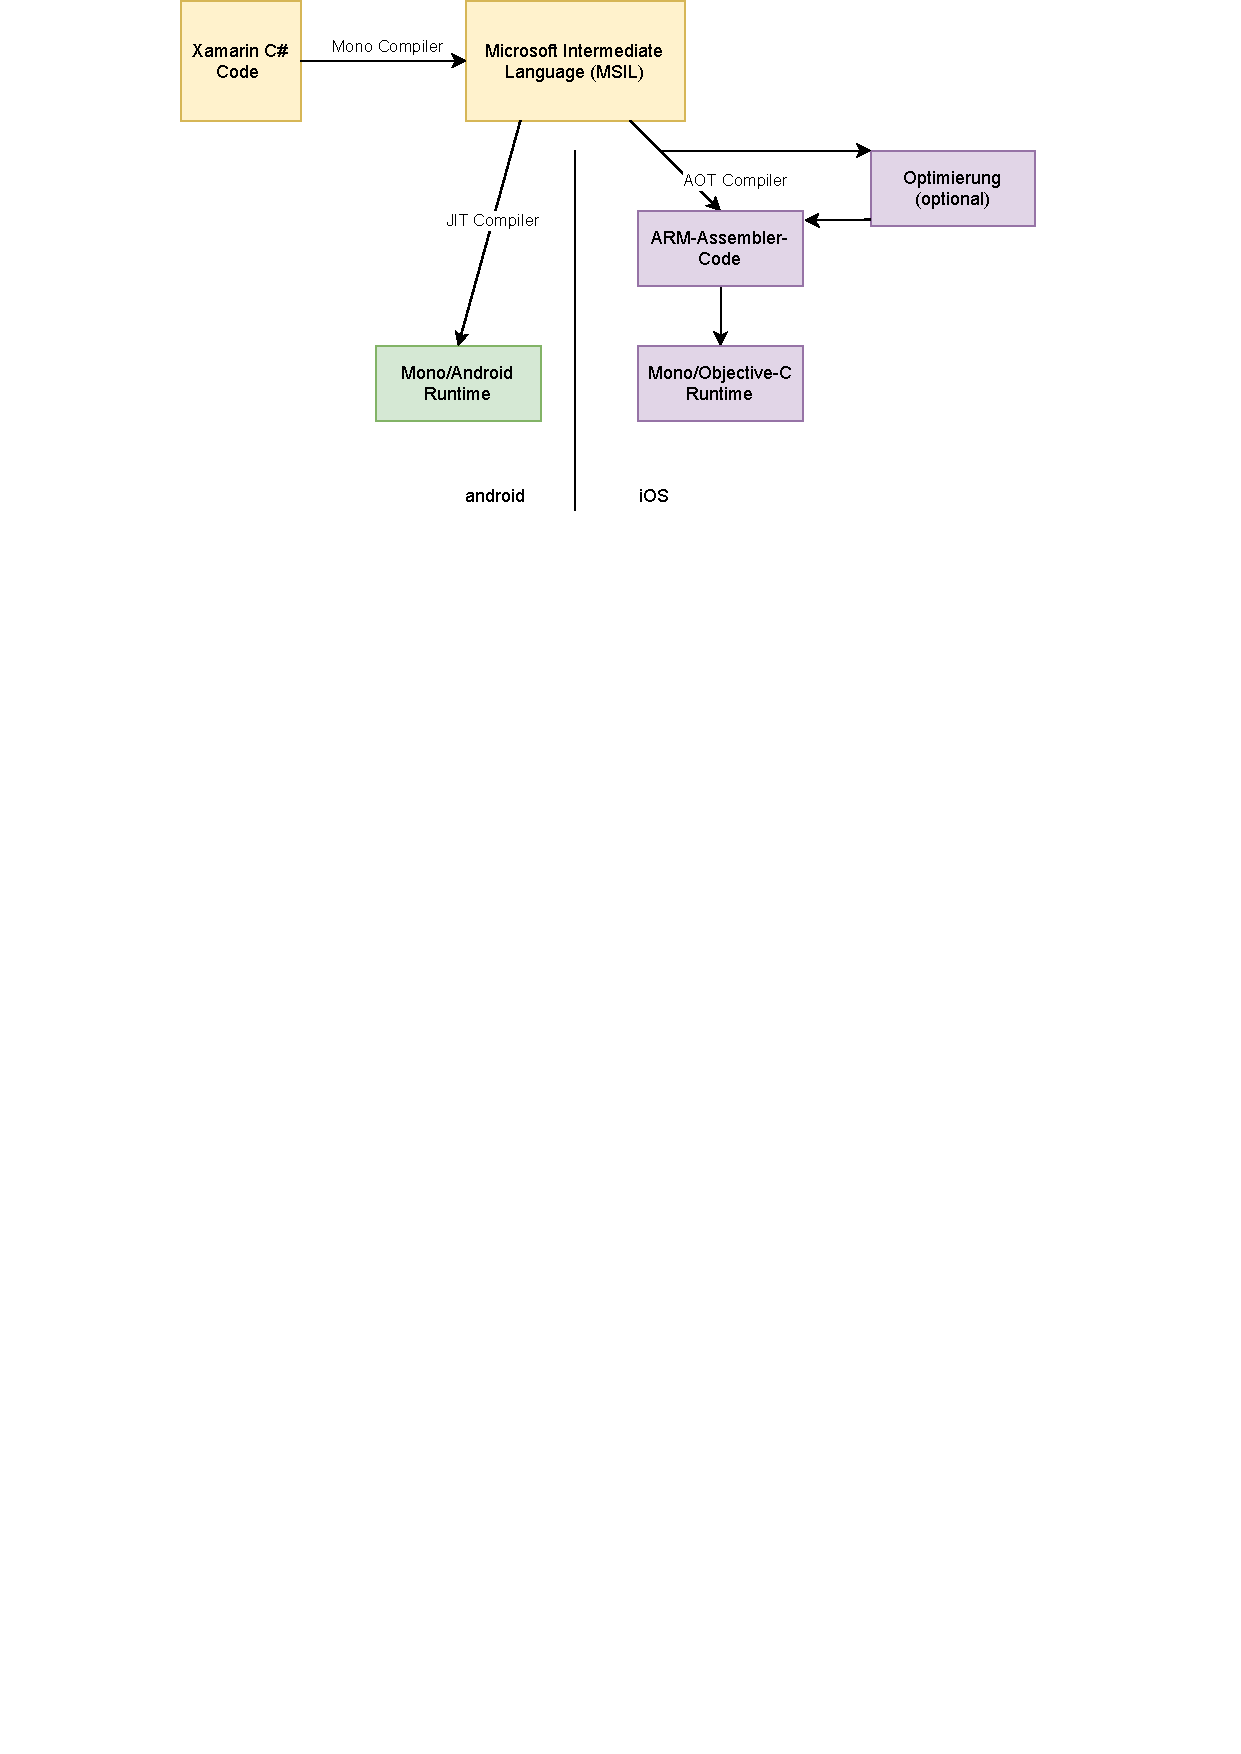
\includegraphics[clip, trim=3cm 20cm 0 0, width=1.2\textwidth]{xamarin_build.pdf}
    \caption{Buildprozess einer Xamarin-Anwendung für die Plattformen Android und iOS}
    \label{fig:xamarin_build}
\end{figure}




Unabhängig von der aktuellen Plattform, hat eine Xamarin-Anwendung immer Zugriff auf die bekannten .NET \acp{API}, wie bereits in \autoref{fig:architecture_xamarin} gezeigt.
Darüber hinaus ist ein Zugriff auf die \acp{SDK} der Plattformen möglich, wodurch kein komplexes Plugin-System für den Zugriff auf native \acp{API} benötigt wird.
Durch die parallele Ausführung einer nativen Ausführungsumgebung ist es außerdem möglich, auf beliebigen nativen Code zuzugreifen.
Damit können bereits vorhandene Bibliotheken oder Drittanbieter-Bibliotheken in die Anwendung integriert werden \cite{Xamarin_Einfuehrung}.
\newline
Ein großes Problem von Xamarin besteht darin, dass typischerweise für jede Plattform eine eigene native Benutzerschnittstelle entwickelt werden muss.
Das erhöht den Aufwand im Vergleich zu \nameref{sec:Frameworks_Ionic} deutlich.
Mit dem zusätzlichen \ac{UI}-Tool Xamarin.Forms können plattformübergreifende \acp{UI} erstellt und der Entwicklungsaufwand somit noch weiter gesenkt werden.
Vor allem die, für November 2021 geplante, Weiterentwicklung .NET \ac{MAUI} soll Plattformübergreifende Benutzerschnittstellen deutlich verbessern.
Das Ziel dabei ist es, den Anteil des geteilten Codes weiter zu steigern und gleichzeitig Benutzerschnittstellen zu entwickeln, die nicht mit dem nativen Design der jeweiligen Plattform brechen \cite{NET_MAUI}.
Damit soll es möglich sein, bis zu 100 \% des Codes für alle Plattformen gleichermaßen zu verwenden \cite{Nawrocki_Comparison_Hybrid_Native_Frameworks, NET_MAUI, Bakker_Xamarin_XamarinForms_Native}.
Microsoft gibt an, dass \glqq Entwickler durchschnittlich 90 Prozent Ihrer Anwendung plattformübergreifend freigeben [können]\grqq{} \cite{Xamarin_Einfuehrung}.
Der Anteil an geteiltem Code liegt bei \nameref{sec:Frameorks_Cordova}/\nameref{sec:Frameworks_Ionic} ohne zusätzliche Plugins bei 100 \%.
Durch den Einsatz von vielen Plugins kann der Anteil aber deutlich geringer ausfallen.
\newline
\newline
Xamarin-Anwendungen können in einigen Fällen die Performance nativer Anwendungen erreichen.
Allgemein fällt die Performance nur etwas geringer aus \cite{Nawrocki_Comparison_Hybrid_Native_Frameworks, Bakker_Xamarin_XamarinForms_Native, Xamarin_Homepage}.
Allerdings ist die Startzeit von Xamarin-Anwendungen unter Android durch die \ac{JIT}-Kompilierung langsam \cite[S. 42]{Willocx_CrossPlatform_Performance}.
Die Startzeit für iOS-Anwendungen ist zwar deutlich geringer und nur geringfügig langsamer als bei nativen Anwendungen.
Jedoch sind die erzeugten Apps unter iOS um einiges größer als nativ entwickelte Apps.
In einem Beispiel war eine Xamarin-App mehr als 16-mal so groß wie eine vergleichbare native App \cite[S. 23ff.]{Nawrocki_Comparison_Hybrid_Native_Frameworks}.
\newline
%TODO: check
In der letzten Entwickler-Umfrage von StackOverflow \cite{Stackoverflow_2022} gab eine Mehrheit von 54,6 \% der Entwickler, die mit Xamarin arbeiten, an, das Framework nicht weiterhin verwenden zu wollen.
Gleichzeitig wollen 45,4 \% dieser Entwickler, Xamarin auch in Zukunft einsetzen.
Die Beliebtheit von Xamarin kann also eher als ausgeglichen bezeichnet werden.